\documentclass[12pt,letterpaper]{article}
\usepackage[margin=1in]{geometry}
\usepackage{fancyhdr}
\usepackage[utf8]{inputenc}
\usepackage{palatino}
\usepackage{microtype}
\usepackage{hyperref}
\usepackage{graphicx}
\usepackage{lastpage}
\usepackage[hang,small,margin=1in]{caption}
\usepackage{titlesec}

\renewcommand{\headrulewidth}{0pt}
\fancyfoot{}
\fancyfoot[C]{\sffamily Page \thepage\ of \pageref{LastPage}}
\pagestyle{fancy}

\titleformat{\section}{\bfseries\MakeUppercase}{\arabic{\thesection}}{1em}{}
\titleformat{\subsection}{\bfseries}{\arabic{\thesection}.\arabic{\thesubsection}}{1em}{}
\titleformat{\subsubsection}{\itshape}{\arabic{\thesection}.\arabic{\thesubsection}.\arabic{\thesubsubsection}}{1em}{}

\setlength{\parindent}{0cm}
\setlength{\parskip}{1em}

\captionsetup[figure]{labelfont=it, font=it}
\captionsetup[table]{labelfont={it,sc}, font={it,sc}}

\hypersetup{colorlinks, linkcolor = black, citecolor = black, urlcolor = black}
\urlstyle{same}



\begin{document}

\fancyfoot{}
\begin{center}
    \hfill \\
    \vspace{4in}
    {\bf\Huge CS457 Project \#2 \\}
    \vspace{2in}
    {\Large Soo-Hyun Yoo \\ January 16, 2015}
\end{center}

\newpage
\fancyfoot[C]{\sffamily Page \thepage\ of \pageref{LastPage}}

\section*{Source Files}

\begin{itemize}
    \item p2.rib
    \item p2d.sl
    \item p2s.sl
\end{itemize}


\section*{Explanation}

\subsection*{p2.rib}

We declare some of the variables to be used, A, B, Height, and Ramp, as floats.
After setting some output options and light and field of view settings, we set
up our world. The surface and displacement shaders are called with some values
assigned to the variables declared earlier in the file. Default color and
opacity are set, and the world is transformed so the object is beautifully in
view.

\subsection*{p2d.sl, p2s.sl}

The surface and displacement shader files are constructed similarly.

Both begin with definitions of some default values for the input variables.
Ellipse geometry is calculated using the given axis values.

In the surface shader, the distance from the edge of each ellipse, latitude,
and longitude values are used to calculate a HSV color value. Smoothstep is
used to generate a gradient.

In the displacement shader, the same distance is instead used to displace the
surface to a certain height defined by the Ramp variable. As
DISPLACEMENT\_MAPPING is left defined, bump mapping is disabled.


\newpage
\section*{Results}

\begin{figure}[!h]
    \centering
    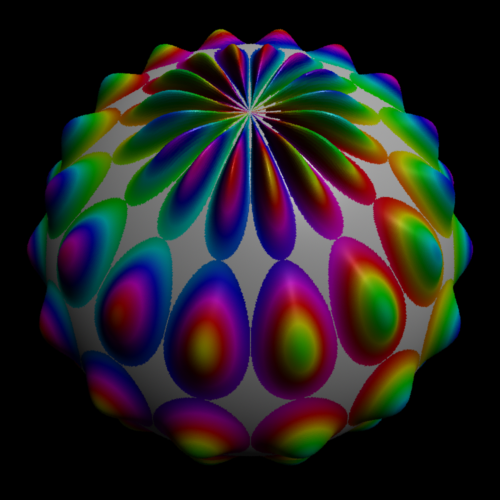
\includegraphics[width=0.5\textwidth]{img/p2_25.png}
    \caption{Rainbow ellipses}
    \label{fig:ellipses}
\end{figure}

\begin{figure}[!h]
    \centering
    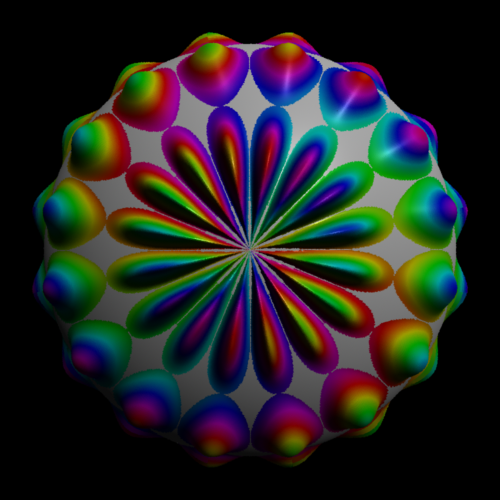
\includegraphics[width=0.5\textwidth]{img/p2_0.png}
    \caption{Rainbow ellipses at pole}
\end{figure}

\begin{figure}[!h]
    \centering
    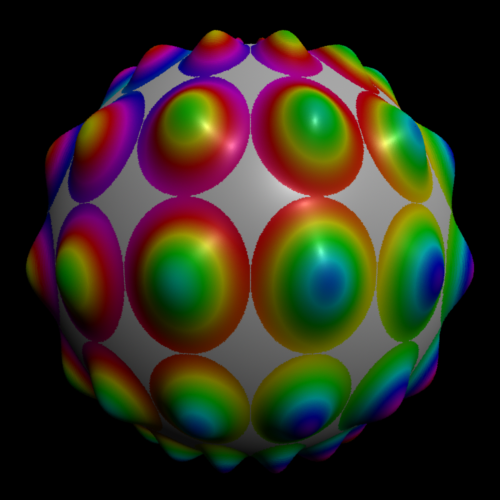
\includegraphics[width=0.5\textwidth]{img/p2_90.png}
    \caption{Rainbow ellipses at equator}
\end{figure}

\begin{figure}[!h]
    \centering
    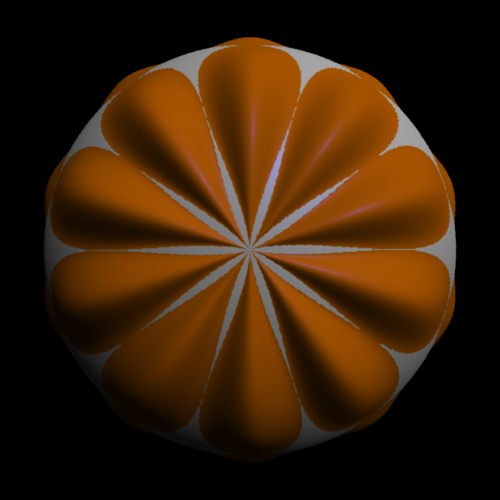
\includegraphics[width=0.5\textwidth]{img/p2_plain0.png}
    \caption{Plain, fatter ellipses at north pole}
\end{figure}

\begin{figure}[!h]
    \centering
    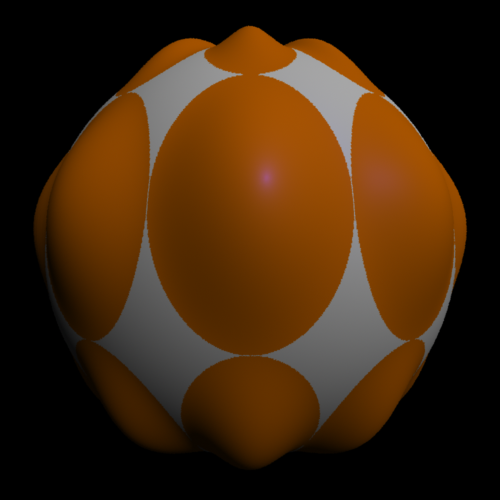
\includegraphics[width=0.5\textwidth]{img/p2_plain90.png}
    \caption{Plain ellipses at equator}
\end{figure}

\begin{figure}[!h]
    \centering
    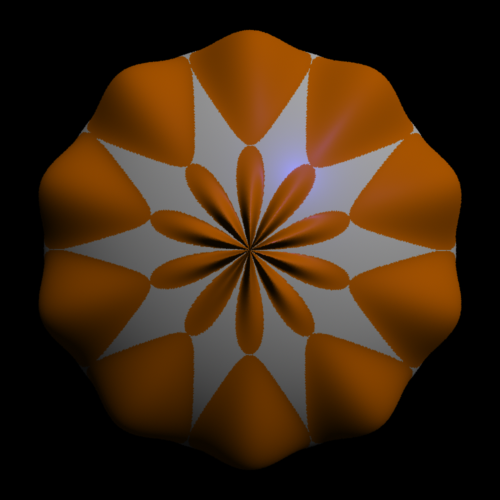
\includegraphics[width=0.5\textwidth]{img/p2_plain180.png}
    \caption{Plain ellipses at south pole. Note that as the vertical diameter
        of these ellipses did not divide evenly into 1, the final ellipses are
        truncated at this pole.}
\end{figure}

\end{document}
